\chapter{Introducción}
\label{cap:introduccion}

La Robótica es uno de los retos tecnológicos más desafiantes a los que se enfrenta el mundo actual. El objetivo principal de esta ciencia es crear máquinas que hagan la vida más fácil, ya sea realizando labores peligrosas o tediosas o simplemente como medio de entretenimiento.\\

En este primer capítulo se explica el contexto en el que se encuadra el proyecto, la robótica. Muchas técnicas de visión artificial son utilizadas por los robots para medir el entorno en el que se encuentran. Extraer información del mundo no es tarea fácil y las mediciones suelen ser bastante imprecisas. Para reducir y, de alguna manera, minimizar estas imprecisiones se utilizan una serie de algoritmos que se verán más adelante. Todos estos términos se exponen en este capítulo. Por último se explica qué es la RoboCup\footnote{http://www.robocup.org}, el porqué de esta competición y la estructura de este documento.

\section{Robótica}
\label{sec:robotica}

La robótica es la rama de la ciencia que estudia los robots. El término \textit{Robot} es difícil de definir. Fue introducido por el escritor checo Karen Capek en su obra teatral R.U.R. (Robots Universales de Rossum), estrenada en 1921, figura \ref{fig:rur}. Esta palabra deriva del término checoslovaco \textit{Robota} que significa literalmente trabajar y, figuradamente, trabajo duro o penoso. \\

\begin{figure}[hbtp]
  \centering
  \subfloat[Un hombre, una mujer y tres robots]{
    \label{fig:rur1}
    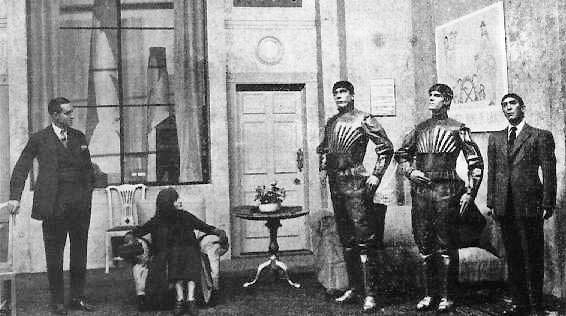
\includegraphics[width=9.3cm]{img/cap1/rur1}
  }
  \subfloat[Rebelión de los robots]{
    \label{fig:rur2}
    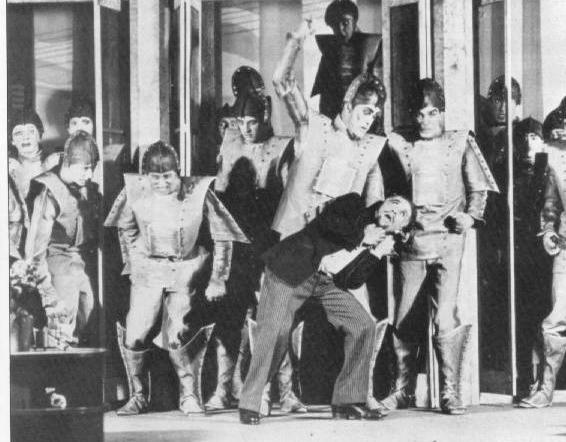
\includegraphics[width=6.7cm]{img/cap1/rur2}
  }
  \caption{Imágenes de distintas representaciones de la obra teatral R.U.R.}
  \label{fig:rur}
\end{figure}

No hay una única definición que satisfaga a todos los organismos internacionales de estandarización. Por ejemplo, la IFR (International Federation of Robotics) utiliza la definición propuesta por la ISO (Organización Internacional para la Estandarización) incluido en el ISO 8373. En este documento se define como \textit{manipulador programable en tres o más ejes, multipropósito, controlado automáticamente y reprogramable}. Esta definición también es usada por otros comités como el EURON (EUropean RObotics research Network). En cambio, la RIA (Robotic Industries Association) define el término robot como \textit{manipulador reprogramable y multifuncional diseñado para mover materiales, partes, herramientas o dispositivos especializados a través de movimientos programados para la realización de una serie de tareas}. Esta definición es un poco más amplia que la anterior. Por último, la RAE define el término robot como \textit{máquina o ingenio electrónico programable, capaz de manipular objetos y realizar operaciones antes reservadas sólo a las personas}.\\

Como se puede comprobar, cada una de las definiciones de robot es distinta de las otras. En mi opinión, la definición contenida en la ISO 8373 y la dada por la RIA están muy centradas en la robótica industrial. De hecho, se define al robot como un manipulador. En el lado opuesto, la definición proporcionada por la RAE es demasiado amplia y abstracta. A mi juicio, un robot es una máquina programable capaz de interactuar con su entorno, ya sea modificándolo directamente ya desplazándose por él, para realizar una o varias tareas. Las tareas asignadas suelen ser aquellas que por su peligrosidad, repetición o precisión suponen una liberación para las personas.\\

Desde siempre, el ser humano ha intentado construir máquinas que le liberen, simplifiquen o faciliten el trabajo. Los antiguos egipcios unieron brazos mecánicos a las estatuas de sus dioses y los griegos construyeron estatuas con sistemas hidráulicos. Estas estatuas automatizadas eran utilizadas para atemorizar, fascinar e infundir respeto al pueblo. Estos inventos pueden considerarse como los primeros \textit{''robots''} de la historia, aunque distan mucho de los robots actuales.\\

El inicio de la robótica, tal y como la vemos en estos momentos, puede fijarse en el siglo XVIII. En 1801 el francés Joseph Jacquard inventó un telar mecánico programable mediante tarjetas perforadas, figura \ref{fig:telar-jacquard-general}. Esta máquina permitía elaborar diseños de telares complejos a usuarios inexpertos. Cada tarjeta perforada correspondía a una línea del diseño y la unión de varias tarjetas formaban un patrón con el que se tejería el telar. En esta época también se construyeron algunos artilugios curiosos, como una muñeca mecánica capaz de hacer dibujos de forma autónoma, inventada por Henri Maillardert, o unos músicos de tamaño humano creados por Jacques de Vauncansos. Estos \textit{''robots''} tenían un propósito más de ocio que laboral.\\

\begin{figure}[htbp]
  \centering
  \subfloat[El telar de Jacquard.]{
    \label{fig:telar-jacquard}
    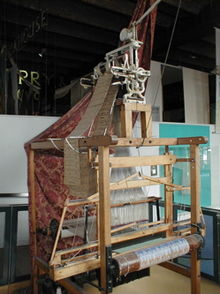
\includegraphics[width=8cm]{img/cap1/telar-jacquard}
  }
  \subfloat[Tarjeta programable del telar.]{
    \label{fig:tarjeta-jacquard}
    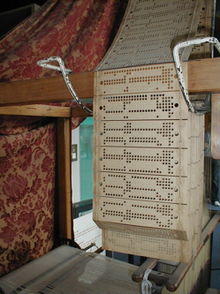
\includegraphics[width=8cm]{img/cap1/tarjeta-jacquard}
  }
  \caption{El telar de Jacquard está expuesto en el Museo de la ciencia y la industria en Manchester, Inglaterra.}
  \label{fig:telar-jacquard-general}
\end{figure}

Pero no fue hasta mediados del siglo XX, gracias a los avances en inteligencia artificial, cuando se crearon los primeros robots modernos. El primer robot industrial programable se construye e instala en 1961 en la \textit{Ford Motors Company}, se llamaba \textit{Unimate}. Su cometido era el levantar piezas industriales que estaban a altas temperaturas. Sin embargo, es en la década de 1970 cuando comienza a desarrollarse completamente la robótica. En 1973 aparece el primer robot con 6 ejes electromecánicos, figura \ref{fig:famulus} y, a los pocos años, el primer brazo mecánico programable, figura \ref{fig:puma}. Estos primeros robots modernos eran básicamente manipuladores, es decir, brazos mecánicos fijos en el suelo que realizan una tarea concreta.\\

\begin{figure}[hbtp]
  \centering
  \subfloat[FAMULUS]{
    \label{fig:famulus}
    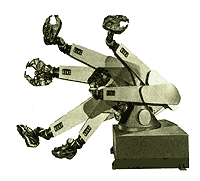
\includegraphics[width=8cm]{img/cap1/famulus}
  }
  \subfloat[PUMA]{
    \label{fig:puma}
    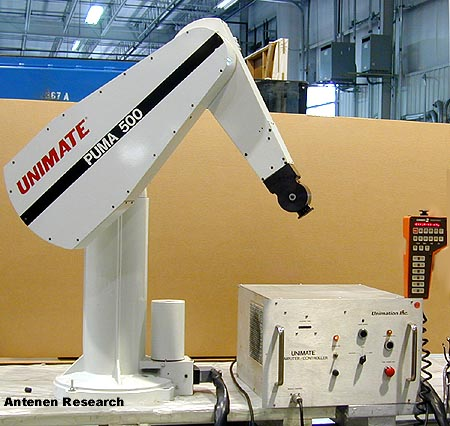
\includegraphics[width=8cm]{img/cap1/puma}
  }
  \caption{Dos de los primeros robots programables en la década de 1970.}
\end{figure}

Los robots definen su funcionalidad y características en función de una serie de elementos hardware. Estos elementos son los encargados de recibir estímulos, procesarlos y efectuar una respuesta. Los elementos hardware se clasifican en sensores, actuadores y procesadores: 

\begin{itemize}
  \item \textbf{Sensores.} Son dispositivos que miden propiedades del entorno tales como distancia, temperatura, intensidad lumínica o señal GPS entre otros. También existen los sensores propioceptivos que miden propiedades del robot, como puede ser la temperatura de los motores, para prevenir que se quemen, o el número de vueltas que da una rueda. Los sensores más utilizados son: 
    \begin{enumerate}
      \item \textbf{Ultrasonido.} Es un dispositivo que sirve para medir distancias. La distancia se calcula midiendo el tiempo de vuelo de una onda sonora. En otras palabras, se calcula el tiempo que tarda la onda en ir y volver después de rebotar en un obstáculo. Conocido el tiempo de vuelo y la velocidad de la onda, la distancia se calcula por medio de una sencilla operación matemática. La onda se emite por encima del espectro audible por el ser humano. Su uso se limita a interiores y el error en la medición suele ser de aproximadamente el 1\% de la distancia medida. 
      \item \textbf{Láser.} El láser también sirve para medir distancias y ésta se calcula de la misma manera que lo hace el ultrasonido, sólo que, en vez de utilizar una onda sonora, utiliza una frecuencia de luz del espectro no visible. Este dispositivo es más preciso que el ultrasonido, puede utilizarse tanto en interiores como en exteriores y el error en las medidas suele ser de apenas unos pocos milímetros, pero también es bastante más caro. Un ultrasonido tiene un precio del orden de decenas de dólares, mientras que un láser tiene un precio de miles de dólares.
      \item \textbf{Cámara.} Este sensor es uno de los más populares. En un sensor muy rico y barato, el único problema de este dispositivo es la dificultad de interpretar las imágenes por el costo computacional que conlleva dicha tarea. En el siguiente apartado de visión computacional en robots se habla más en profundidad de estos dispositivos.
  \end{enumerate}
En la figura \ref{fig:nao-laser} se puede ver al robot Nao equipado con un láser en la cabeza, aunque este dispositivo es opcional. El robot también dispone de ultrasonidos en el pecho, colocados en la banda azul que rodea el botón central, y de dos cámaras, colocadas una en la frente y la otra en la boca.

\begin{figure} [hbtp]
  \begin{center}
    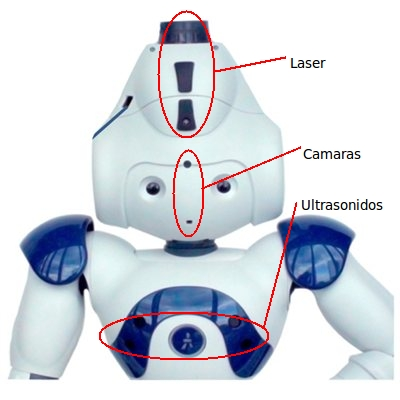
\includegraphics[width=9cm]{img/cap1/nao-laser}
  \end{center}
  \caption{Robot Nao equipado con un láser en la cabeza.}
  \label{fig:nao-laser}
\end{figure}

\item \textbf{Actuadores.} Son dispositivos que modifican el estado del robot o su entorno. Los manipuladores o brazos robóticos son un ejemplo de actuadores que pueden interactuar con el entorno, pero también lo son los altavoces o los LEDs. Es importante destacar en este punto la existencia de dos grandes familias de robots: los robots fijos y los robots móviles. Los robots fijos suelen encontrarse en la robótica industrial. Los robots móviles, como su nombre indica, son aquellos capaces de desplazarse por el entorno.

\item \textbf{Procesadores.} Son elementos encargados de procesar los datos obtenidos de los sensores, analizarlos, comprenderlos y generar una respuesta que ejecutarán los actuadores. Comparando un robot con una persona y haciendo una analogía simple, se puede decir que los sensores, actuadores y procesadores son, respectivamente, los sentidos, los músculos y el cerebro.
\end{itemize}

\section{Visión computacional en robótica}
\label{sec:visionartificialenrobotica}

La visión computacional es el campo de la inteligencia artificial que pretende obtener información del mundo a partir de una o varias cámaras. La cantidad de información que se puede extraer de las imágenes generadas por las cámaras es enorme. Se pueden reconocer objetos, recrear escenas en 3D, seguir personas, etc. Realizar todas estas tareas para un ser humano es muy sencillo, pero para una computadora, en cambio, es una tarea muy difícil.\\

El comienzo de la visión computacional fue marcado por Larry Roberts en 1961, cuando creó un programa que podía \textit{ver}. Esta aplicación era capaz de procesar una imagen de una estructura de bloques y reproducir esa misma estructura desde otra perspectiva. Para ello utilizaba solamente una cámara y un ordenador, pero las condiciones del entorno de las pruebas eran muy limitadas. Muchos científicos de la época trataron de solucionar el problema y se dieron cuenta de que no era tarea fácil. Fue entonces cuando se abrió un nuevo campo de investigación: la visión computacional.\\

Un computador puede tardar años en resolver tareas que para una persona son sencillas y automáticas. A pesar del alto precio computacional que se paga al utilizar las cámaras como fuente de datos, si se consigue analizar correctamente la imagen, es posible extraer mucha información que no podría obtenerse con ningún otro tipo de sensores.\\

A comienzos de la década de 1990 comenzaron a aparecer ordenadores capaces de procesar suficientemente rápido las imágenes. Esto hizo que grandes problemas de visión comenzaran a dividirse en subproblemas más específicos y, por tanto, más sencillos de resolver. Actualmente la visión computacional se utiliza en muchos procesos científicos, militares o industriales para el reconocimiento de objetos o seguimiento de éstos.\\

\begin{itemize}

\item \textbf{Reconocimiento de objetos.} Mediante algoritmos de reconocimiento de objetos se buscan características o patrones de los objetos y se determina si el objeto se encuentra en la imagen o no. Las características más utilizadas son la forma o el color, pero podría utilizarse cualquier otro patrón. En la figura \ref{fig:reconocimientocara} se puede ver un patrón de puntos característicos de la cara de una persona. Al convertir este patrón de puntos en una imagen se pueden detectar caras e incluso reconocer a la persona. 

\item \textbf{Seguimiento de objetos.} Una vez detectado un objeto, se pueden realizar tareas de seguimiento de éste. En el siguiente apartado se verá con mayor detalle este tipo de algoritmos. El procesado iterativo de los objetos detectados permite realizar operaciones más complejas. Por ejemplo, en deportes como el tenis o el cricket se utiliza un sistema informático para hacer el seguimiento de la bola. Este sistema genera una imagen de la trayectoria de la bola que puede ser utilizada  por los jueces para decidir jugadas dudosas. En la figura \ref{fig:seguimientopelota} se puede ver dicha trayectoria. Este sistema es conocido como \textit{Ojo de Halcón}\footnote{http://es.wikipedia.org/wiki/Ojo\_de\_Halcón}.

\end{itemize}

\begin{figure}[h]
  \centering
  \subfloat[Reconocimiento de cara en imagen]{
    \label{fig:reconocimientocara}
    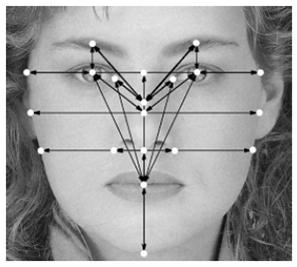
\includegraphics[width=7.6cm]{img/cap1/reconocimiento_cara}
  }
  \subfloat[Seguimiento de la pelota durante un partido de tenis]{
    \label{fig:seguimientopelota}
    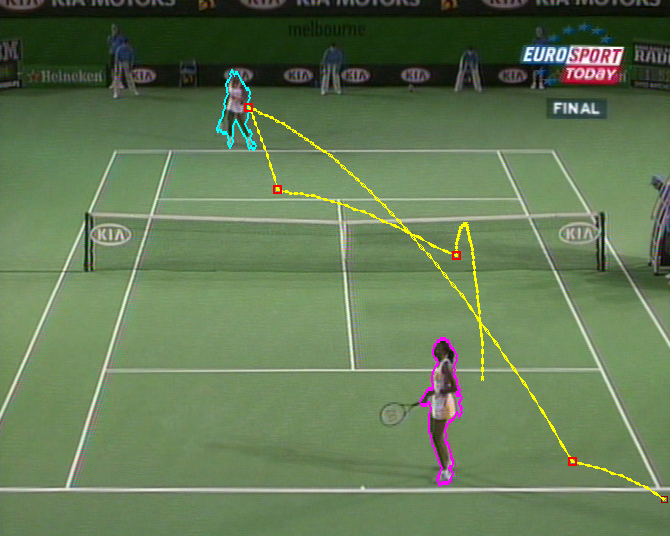
\includegraphics[width=8.4cm]{img/cap1/seguimiento_pelota}
  }
\end{figure}

A pesar de la complejidad que supone obtener información a partir de imágenes, las cámaras son uno de los sensores más utilizados en la robótica. Es un sensor bastante barato comparado con el resto de sensores disponibles y la cantidad información que se puede sacar de una sola imagen es enorme.\\

Los problemas de visión computacional poseen una complejidad bastante elevada. Por ello se han dividido en subproblemas más pequeños, lo que facilita su resolución. Las dos tareas principales para elaborar algoritmos más fiables y robustos son la detección de objetos y el seguimiento o \textit{tracking} de estos. \\

La detección de objetos consiste en localizar un objeto a partir de una imagen. Dependiendo de la resolución de la imagen, esta tarea puede ser muy lenta y consumir muchos recursos. En sistemas de tiempo real, donde se tienen que analizar muchas imágenes por segundo, el tiempo que lleva analizar una imagen es crucial. Si se utilizan sistemas de visión estándar, para conseguir una percepción reactiva del entorno se necesitan un mínimo de aproximadamente 10 imágenes por segundo. Lo ideal sería conseguir una tasa 25 - 30 imágenes por segundo. También hay sistemas más precisos que 
llegan a analizar 60 o más imágenes en un segundo. En la figura \ref{fig:tracking-people} se puede ver una captura de pantalla de un sistema de videovigilancia capaz de detectar y seguir personas en una zona de un aeropuerto utilizando las imágenes de las cámaras de seguridad.\\

\begin{figure} [h]
  \begin{center}
    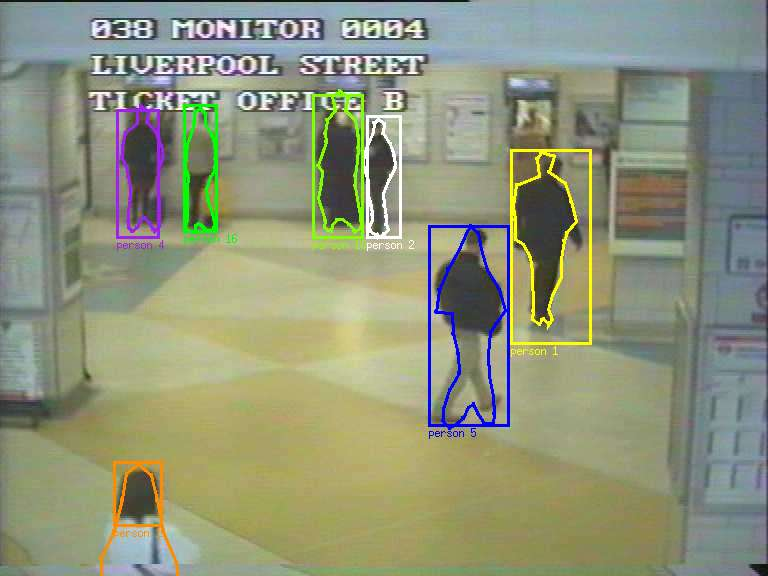
\includegraphics[width=9cm]{img/cap1/tracking-people}
  \end{center}
  \caption{Detector de personas utilizando una cámara de seguridad en un aeropuerto.}
  \label{fig:tracking-people}
\end{figure}

Los detectores devuelven información sobre los objetos interesantes de la imagen. Esta información, dependiendo del tipo de sistema, es más o menos precisa. Por ejemplo, no es lo mismo detectar personas con cámaras de vigilancia en un aeropuerto, donde cada persona es totalmente distinta a otra, que detectar objetos simples en una cadena de montaje de una fábrica, donde la diferencia entre los objetos es mínima. Por este motivo las observaciones suelen llevar asociada una incertidumbre o ruido. La incertidumbre depende de la calibración de los parámetros intrínsecos y extrínsecos de la cámara, condiciones de iluminación, etc. Dicho de otra manera, el ruido asociado a una observación indica el grado de fiabilidad de ésta. Cuanto menor es el ruido, más fiable es la observación y más probabilidades tiene el objeto de encontrarse realmente en la posición marcada. Por el contrario, si el ruido es muy grande, la observación no es fiable y seguramente el objeto se encuentre dentro de un área con centro en la posición marcada donde según te alejas de él, la probabilidad disminuye. También hay que tener en cuenta la aparición de falsos positivos y falsos negativos, que significa detectar un objeto cuando en realidad no hay nada y no detectar el objeto cuando en realidad sí que se encuentra en la imagen, respectivamente. \\

En ocasiones, a partir de las observaciones devueltas por los detectores se puede inferir información que no se encuentra en la imagen, no se ha detectado correctamente o es indistinguible. Para ello es necesario tener un modelo del objeto con el que poder comparar. De esta forma se puede sacar información de objetos que están parcialmente ocultos, información que no es medible directamente, o diferenciar objetos totalmente iguales. Por ejemplo, si se detectan tres vértices de un cuadrado y el cuarto no es localizado \cite{rocapal}, se puede inferir su posición para en otro momento comprobar si de verdad se encuentra en esa posición; o, por ejemplo, se puede medir la velocidad de un objeto a partir de su posición en distintos instantes de tiempo. \\

Para mejorar los algoritmos de detección y obtener datos más fiables surgen los algoritmos de seguimiento. Éstos ayudan notablemente a minimizar los problemas que se acaban de exponer: reducir el ruido de las observaciones, protegerse frente a falsos positivos y negativos, inferir datos nuevos a partir de otros o distinguir objetos cuando son exactamente iguales. \\

\subsection{Visión 2D y 3D}
\label{subsec:vision2dy3d}

La visión de un robot puede ser en dos o tres dimensiones. Cuando se usa una sola cámara, lo habitual es tener una visión en 2D, aunque existen técnicas para deducir la tercera dimensión que falta. Las imágenes proporcionadas por las cámaras no tienen profundidad y todos los objetos se encuentran en el mismo plano: tienen dos dimensiones. Le ocurre lo mismo a un ser humano cuando guiña un ojo, no es capaz de medir distancias con la misma facilidad que si lo hace con los dos. \\

Una persona, ya sea en una imagen o mirando con un solo ojo, utiliza una serie de técnicas instintivas para hacer una representación mental de la imagen y conocer la posición aproximada de los objetos. Por ejemplo, si analizamos la imagen \ref{fig:calle-de-bruselas}, a pesar de ser en 2D se puede inferir mucha información de la escena utilizando algunas de estas técnicas. 

\begin{figure} [h]
  \begin{center}
    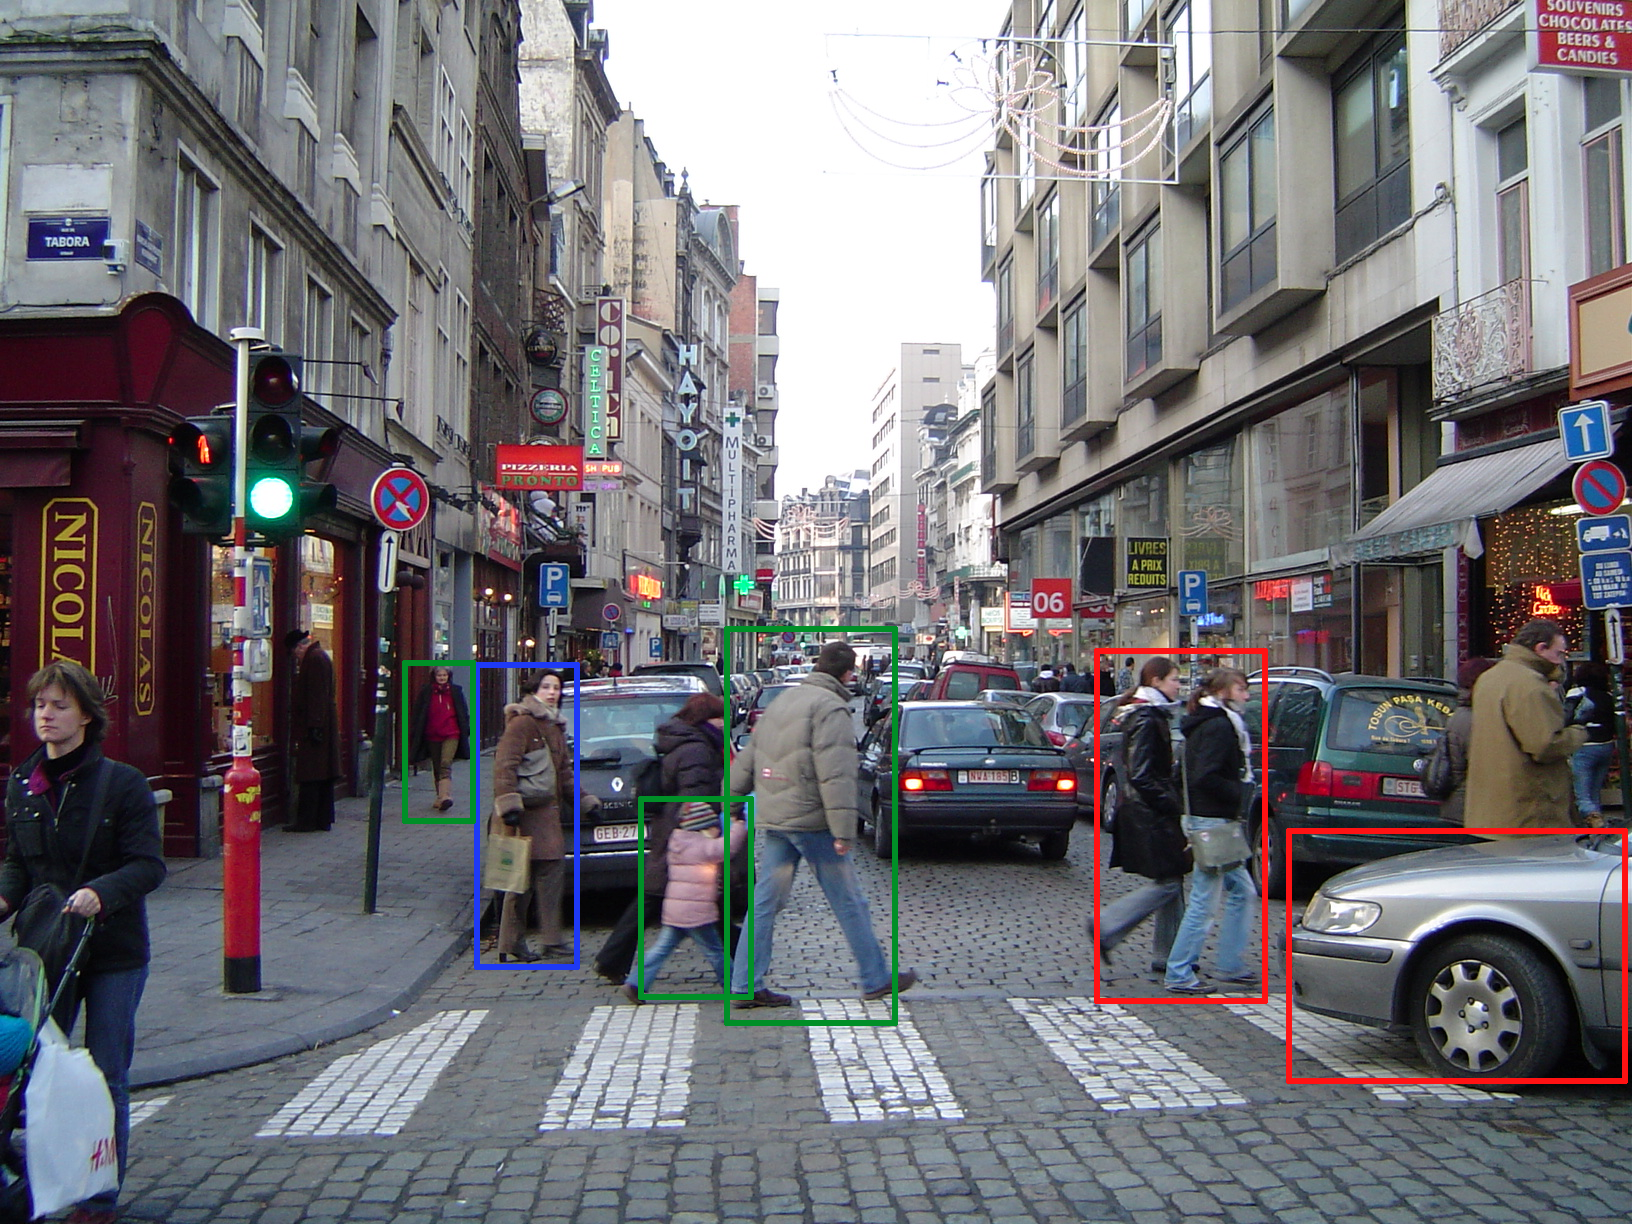
\includegraphics[width=12cm]{img/cap1/calle-de-bruselas}
  \end{center}
  \caption{Imagen de una calle de Bruselas}
  \label{fig:calle-de-bruselas}
\end{figure}

\begin{itemize}

\item En la parte derecha de la imagen se ve el morro de un coche y justo a su izquierda una pareja de mujeres, marcados de color rojo. Se sabe que el coche se encuentra en una posición más cercana porque el punto de intersección de la rueda con el suelo está más abajo en la imagen que los pies de las mujeres.

\item En la parte izquierda de la imagen hay una mujer con una bolsa en la mano rodeada de azul. Se sabe que se encuentra delante del coche porque oculta la vista de éste.

\item De color verde se han resaltado una niña, su padre y una mujer más lejos en la parte izquierda de la imagen. Se sabe que la niña y el padre están más o menos a la misma distancia. De hecho, el padre está un poco más adelantado. Se intuye que es una niña por el color del abrigo y por el tamaño, comparado con el de su padre. En la izquierda de la imagen se puede ver que la mujer tiene el mismo tamaño que la niña; sin embargo, está en una posición más lejana y esto hace que, a pesar de ser más grande en la realidad, su tamaño en la imagen sea menor. Por eso se sabe que se trata de una mujer y no una niña.

\end{itemize}

Estas son solo algunas de las técnicas que se utilizan. Pueden parecer tontas y un poco obvias porque el ser humano lo hace automáticamente y uno no se para a analizarlas, simplemente se saben. Es una capacidad innata de las personas. Para hacer la representación mental de esta imagen se mezcla muchísima información, desde información física de objetos que se conoce \textit{a priori}, como el tamaño y la forma, con información cultural, como el hecho del abrigo rosa. \\

Cuando se quiere tener una visión 3D del entorno, se tienen que utilizar un mínimo de dos cámaras. Las cámaras tienen que estar en una posición conocida con respecto a las otras. Lo más habitual en robots es encontrar un par estéreo de cámaras, donde se colocan las cámaras con una disposición similar a la de los ojos humanos, figura \ref{fig:parestereo}. Las imágenes de las dos cámaras se pueden ver en la figura \ref{fig:stereo2}.

\begin{figure}[h]
  \centering
  \subfloat[Par estéreo]{
    \label{fig:parestereo}
    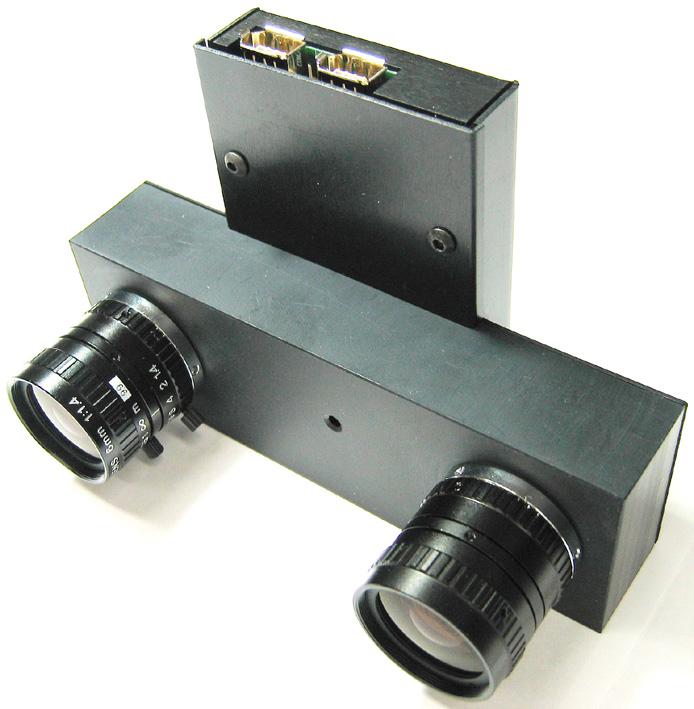
\includegraphics[width=4cm]{img/cap1/stereo}
  }
  \subfloat[Imágenes de un par estéreo de cámaras]{
    \label{fig:stereo2}
    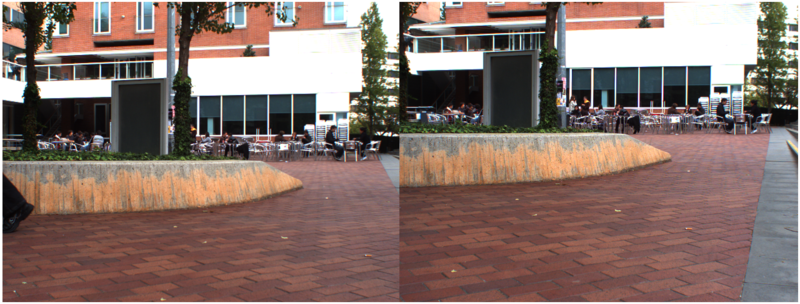
\includegraphics[width=11cm]{img/cap1/stereo2}
  }
\end{figure}

A partir de estas dos imágenes se puede calcular la posición de cualquier punto en la imagen. A partir de un píxel de una de las imágenes hay que descubrir el píxel homólogo en la otra imagen y, mediante un simple cálculo de triangulación, se calcula dicho punto en 3D. La posición calculada es relativa a la posición de las cámaras. El costo computacional del cálculo de estos puntos es bastante alto, pero no hay restricciones en cuanto a la distancia a la que se encuentre el punto, siempre que sea visible en las dos imágenes. \\

En los últimos años ha aparecido un nuevo sensor que está cobrando cada vez más protagonismo en el ámbito de los sensores de robots: la \textit{Kinect}, figura \ref{fig:kinect}. Este dispositivo fue inventando por Microsoft para la videoconsola Xbox 360. Permite controlar e interactuar con la consola sin necesidad de tener contacto físico con un controlador de videojuegos tradicional, como un mando o un joystick. Este dispositivo dispone de una cámara y un sensor de profundidad, que no es más que un proyector de infrarrojos combinado con un sensor CMOS monocromo. Básicamente, lo que hace es medir la distancia para cada píxel de la cámara y así obtener una mapa 3D del entorno, independientemente de la luz ambiental. \\

\begin{figure}[h]
  \centering
  \subfloat[El dispositivo]{
    \label{fig:kinect}
    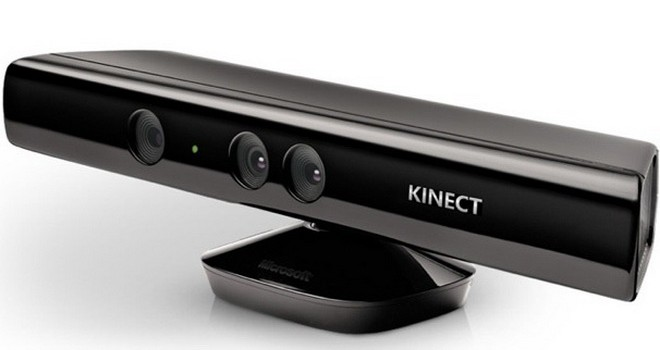
\includegraphics[width=4.5cm]{img/cap1/kinect}
  }
  \subfloat[Imagen e imagen de profundidad]{
    \label{fig:kinect-depth}
    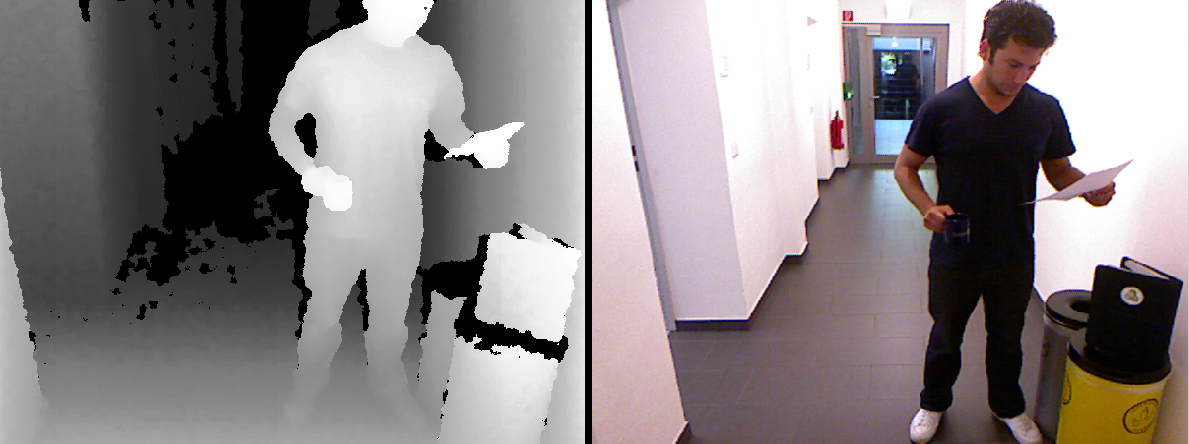
\includegraphics[width=10.5cm]{img/cap1/kinect-depth}
  }
\end{figure}

El cálculo de la matriz de distancias se efectúa al mismo tiempo que se captura la imagen y se hace por hardware, liberando la CPU de ese trabajo. En la figura \ref{fig:kinect-depth} se puede ver la imagen capturada y la matriz de profundidad de la imagen. Cuanto menor es la distancia, más claro es el color del píxel y viceversa. Por este motivo este dispositivo se está haciendo muy popular en robótica en los últimos años. Se consiguen los mismos resultados que con una cámara y un láser a un coste mínimo. Uno de los inconvenientes de los pares estéreos de cámaras es el alto costo computacional del cálculo del píxel homólogo. No es una tarea en absoluto sencilla. En cambio, la \textit{Kinect} tiene esta capacidad para todos los píxeles de la imagen sin costo alguno. Pero también tiene sus limitaciones, su uso se limita prácticamente a interiores. La distancia mínima es de unos 60 centímetros, la distancia máxima de unos 4-5 metros y la luz solar directa sobre el sensor aumenta enormemente el error de las mediciones. \\

\section{RoboCup}
\label{sec:robocup}

La RoboCup\footnote{http://www.robocup.org} es una iniciativa científica a nivel internacional cuyo objetivo es avanzar el estado del arte de la inteligencia en robots. Constituida en 1997, la misión principal era la de crear un equipo de robots completamente autónomos capaz de ganar a la selección de fútbol (humanos) que gane la Copa del Mundo de fútbol en el 2050. Desde que se creó, esta competición se ha expandido y ahora también abarca distintos dominios donde la robótica puede ser aplicada y ser potencialmente útil para la sociedad moderna. \\

La RoboCup está diseñada para entender y encontrar soluciones a problemas complejos del mundo real en un dominio limitado, para que ello sea asequible y computacionalmente posible. En la RoboCup se cubren muchas áreas de investigación que tienen que ver con la inteligencia artificial y la robótica. Entre ellas se encuentran las siguientes: procesamiento en tiempo real, comportamiento reactivo, aprendizaje, planificación, sistemas multi-agente, visión y muchas más. Las competiciones son: \\

\begin{itemize}

\item \textbf{RoboCupSoccer.} Es una competición de fútbol en la que equipos de robots completamente autónomos y cooperativos compiten entre ellos en un partido de fútbol.

\item \textbf{RoboCupRescue.} Competición dónde los robots asisten a \textit{servicios de emergencia} para salvar gente y llevar a cabo tareas peligrosas. Estos robots tiene una gran movilidad, son semi-autónomos y capaces de cartografiar y moverse a través de entornos complejos.

\begin{figure}[h]
  \centering
  \subfloat[RoboCupSoccer]{
    \label{fig:robocupsoccer}
    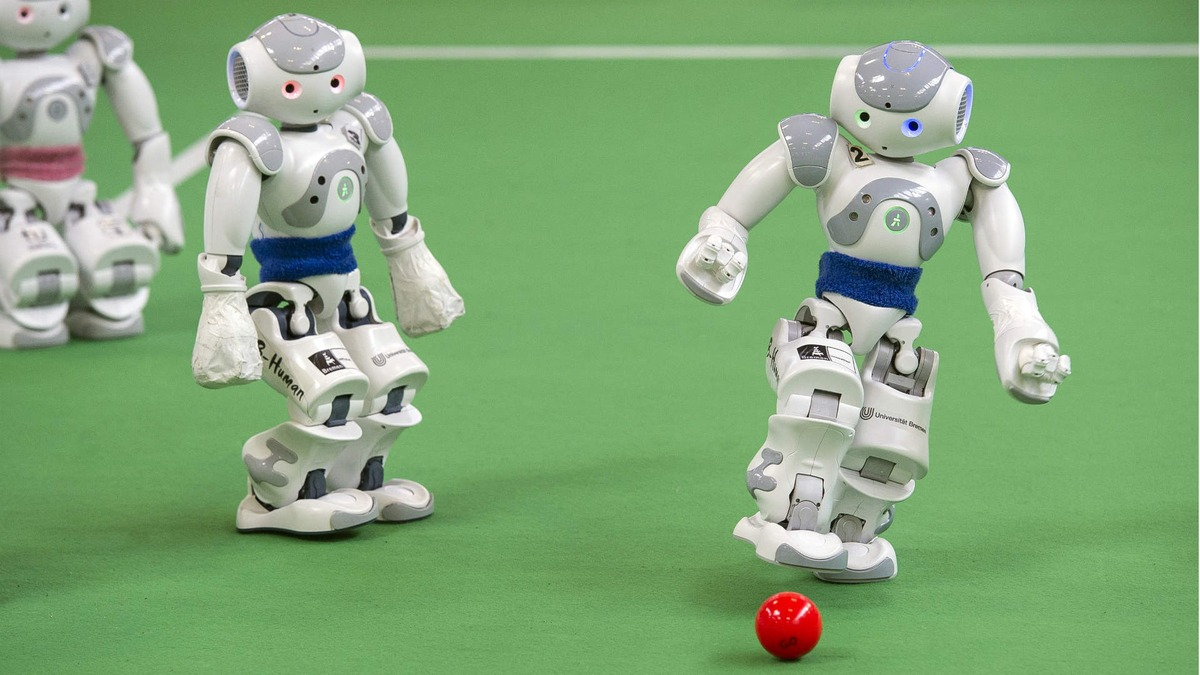
\includegraphics[width=8.1cm]{img/cap1/robocupsoccer}
  }
  \subfloat[RoboCupRescue]{
    \label{fig:robocuprescue}

    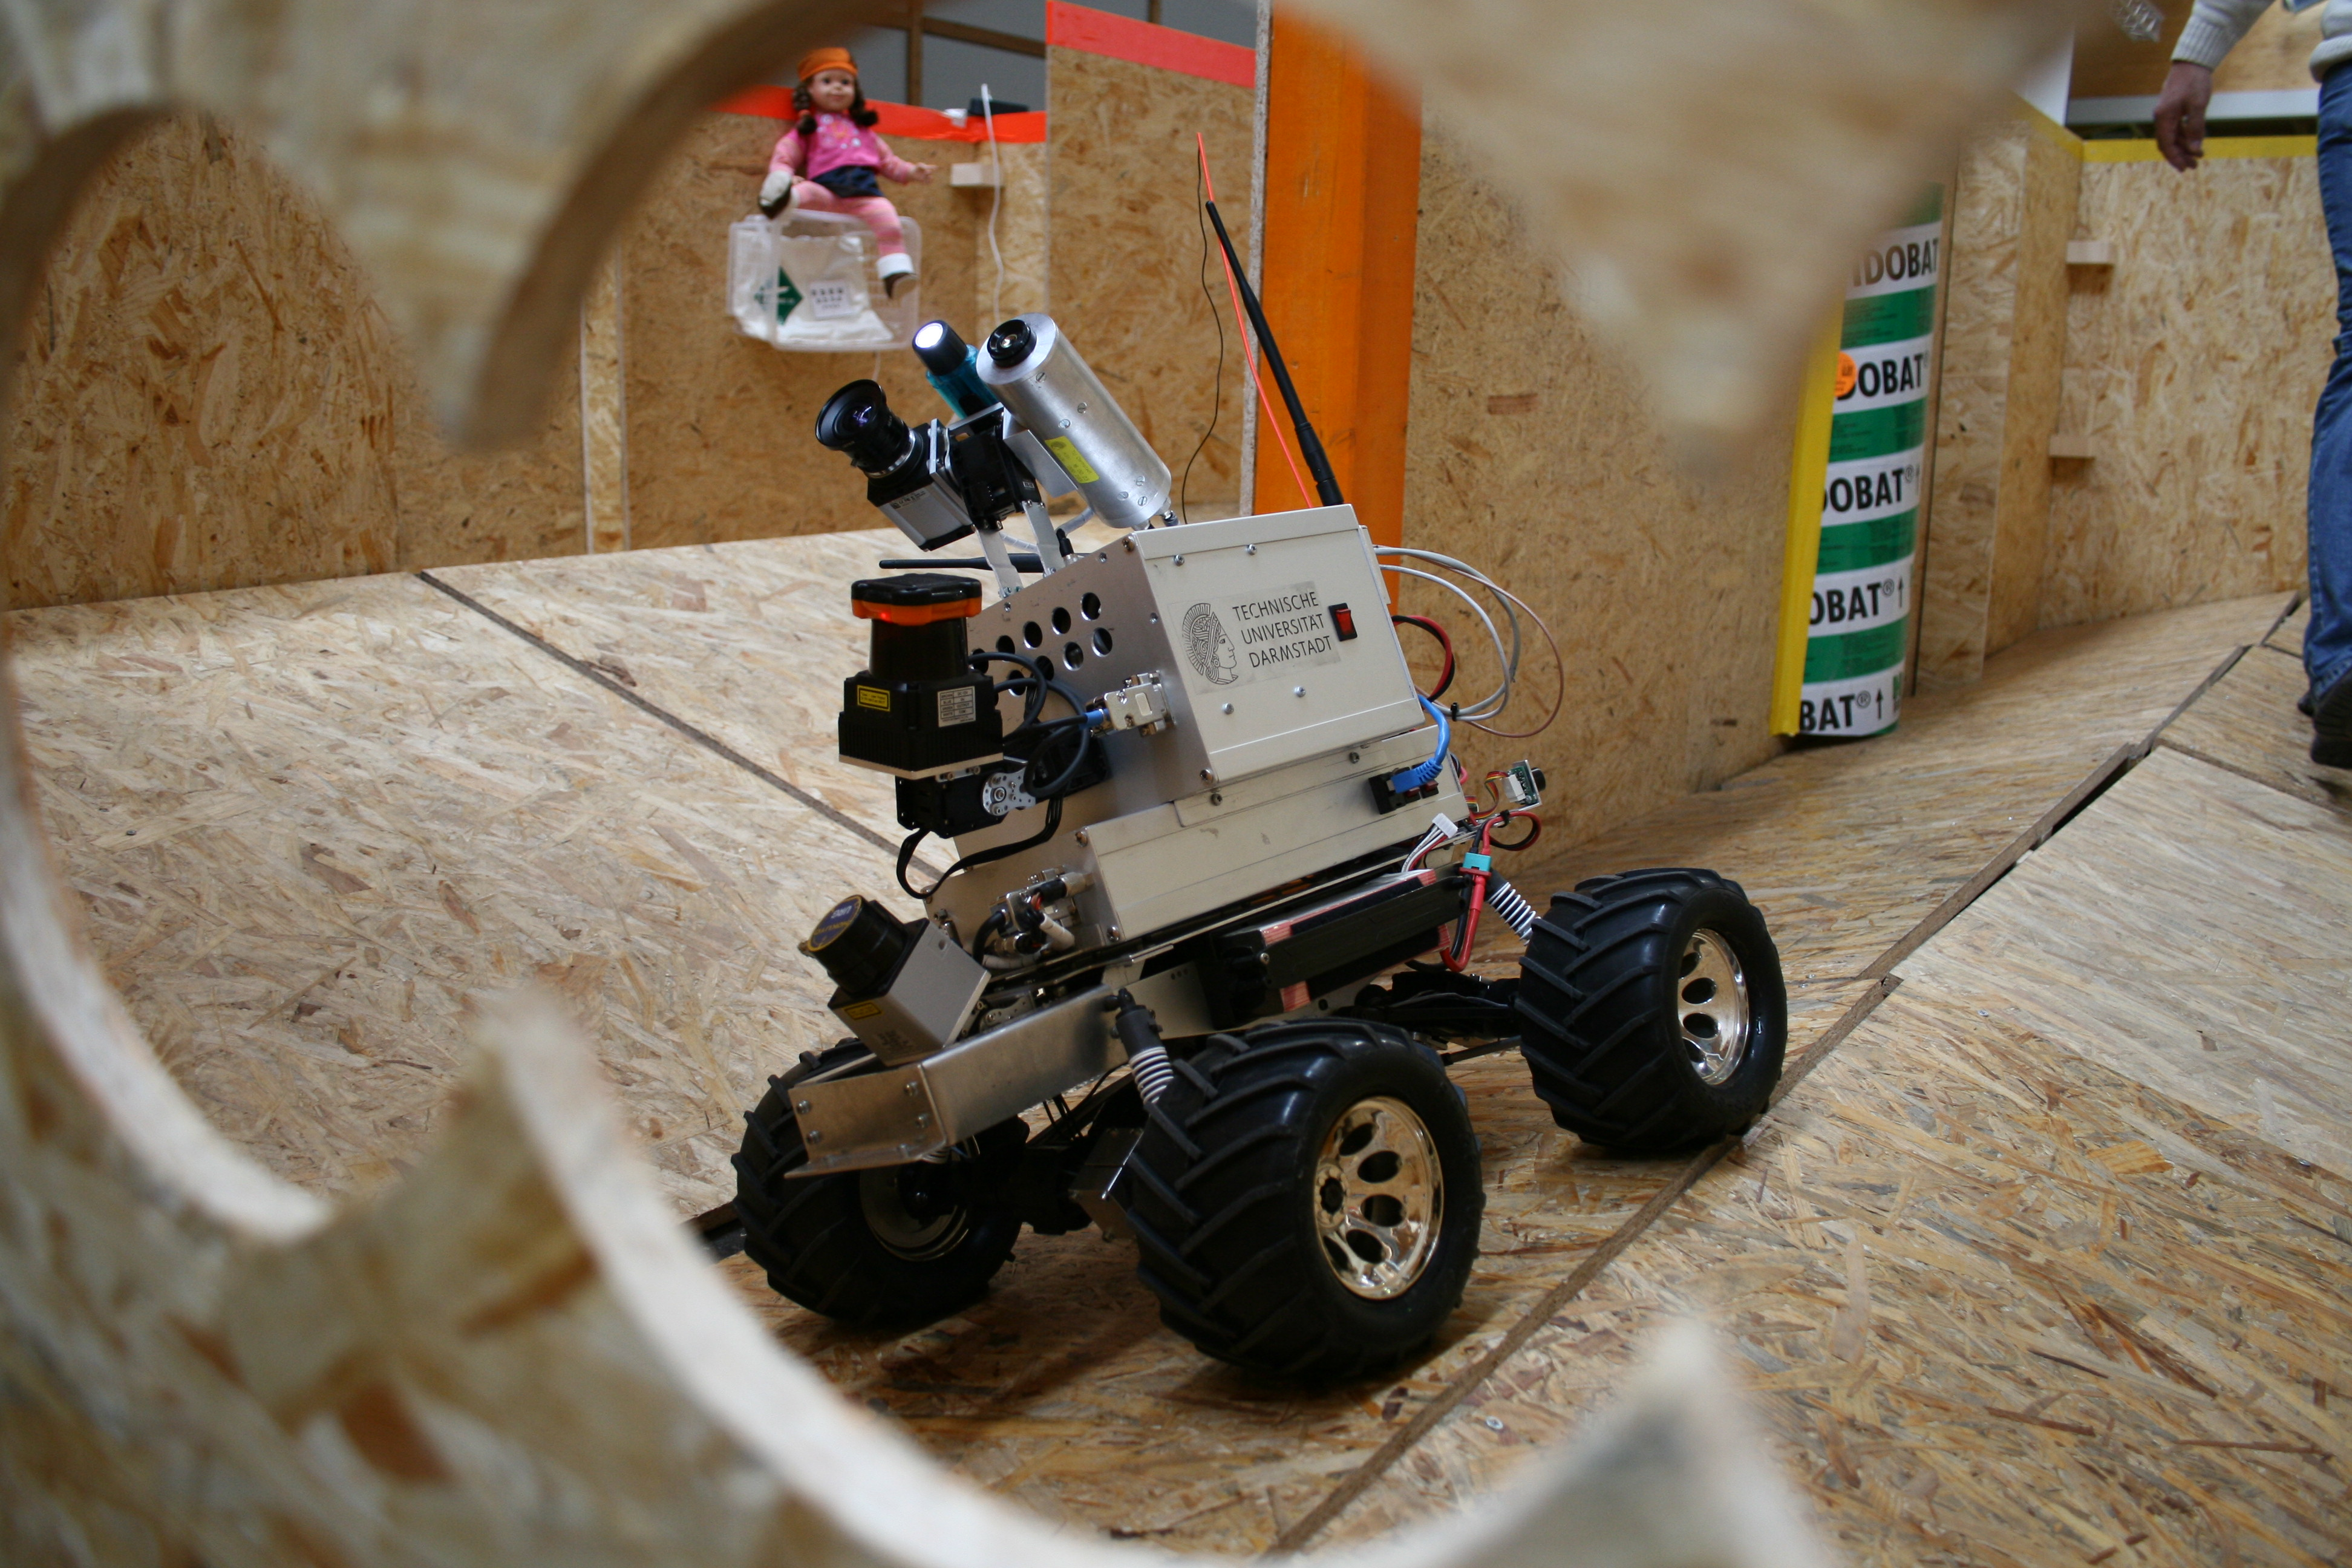
\includegraphics[width=6.9cm]{img/cap1/robocuprescue}
  }
\caption{Competiciones en la RoboCup}
\end{figure}

\item \textbf{RoboCup@Home.} El objetivo de esta competición es realizar típicas tareas domésticas con robots autónomos y una fácil interacción humano-robot.

\item \textbf{RoboCupJunior.} Esta competición se centra en los más jóvenes. Los participantes tienen que construir y programar robots autónomos sobre los que tienen que aplicar la tecnología, ingeniería y las matemáticas sobre las que se sustenta la robótica.

\begin{figure}[h]
  \centering
  \subfloat[RoboCupH@me]{
    \label{fig:robocuphome}
    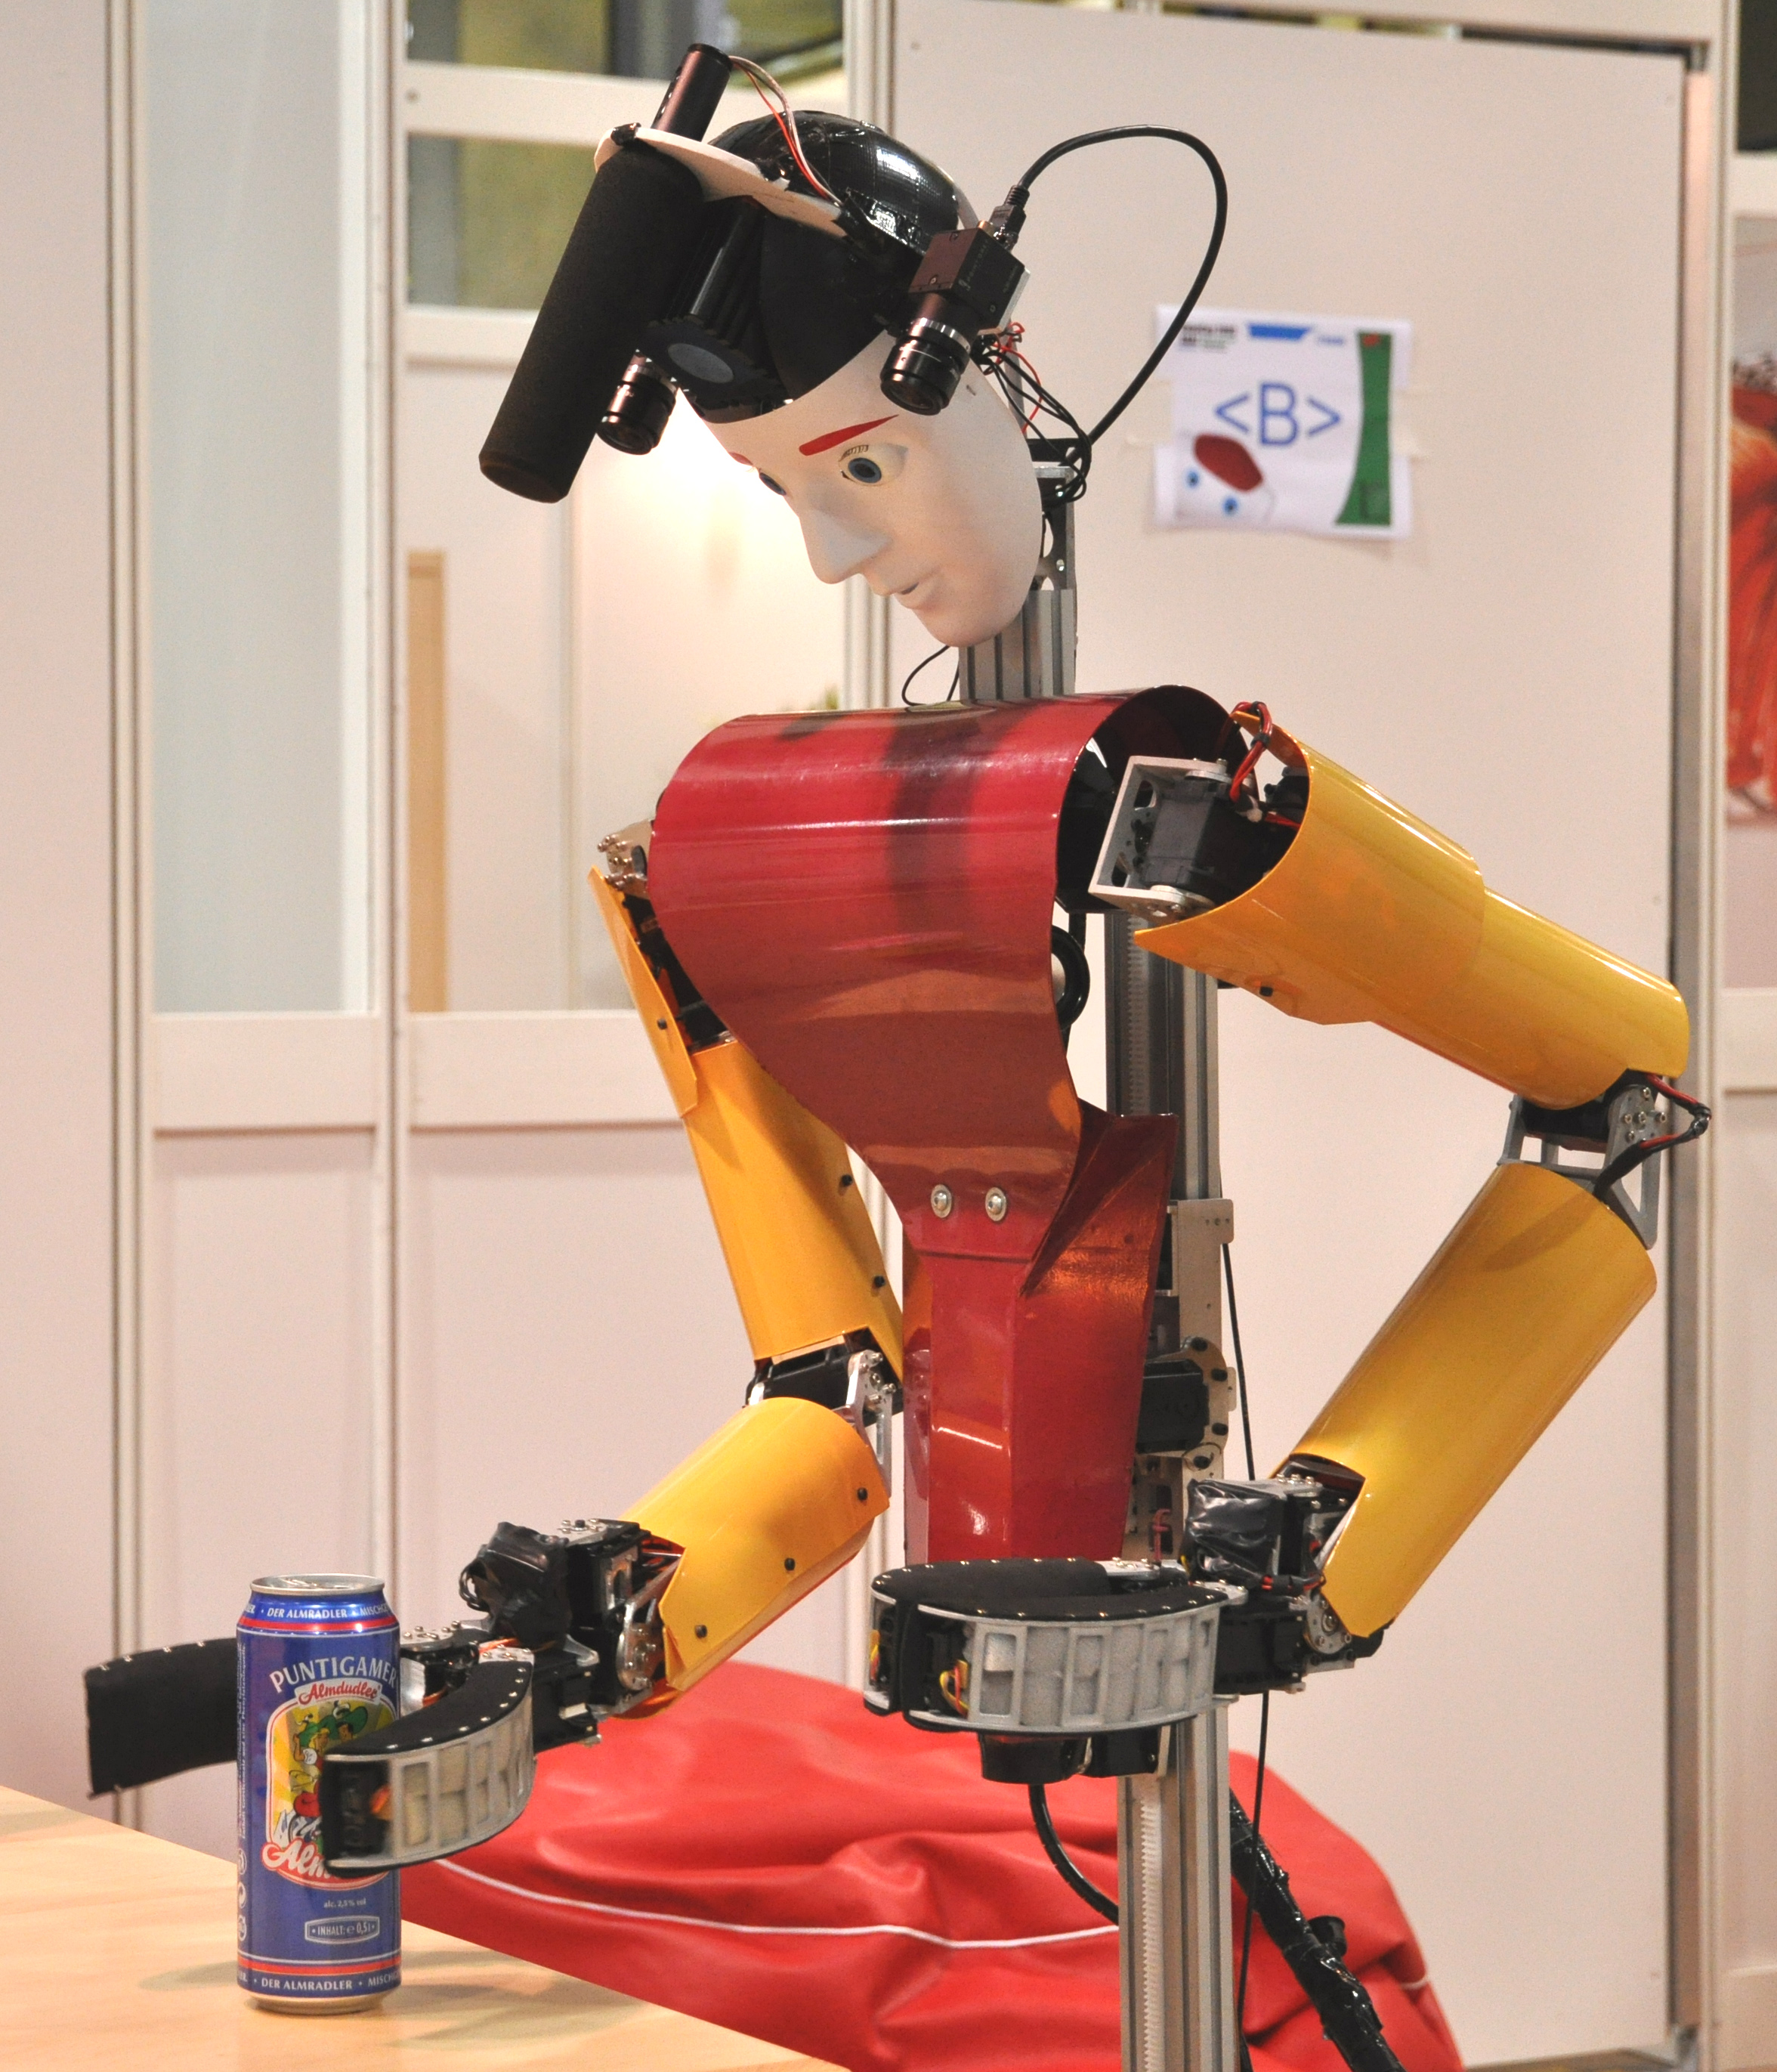
\includegraphics[width=5.9cm]{img/cap1/robocuphome}
  }
  \subfloat[RoboCupJunior]{
    \label{fig:robocupjunior}
    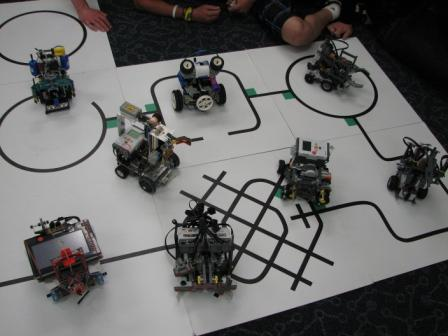
\includegraphics[width=9.1cm]{img/cap1/robocupjunior}
  }
\caption{Competiciones en la RoboCup}
\end{figure}

\end{itemize}

La gran pregunta respecto a esta competición es ¿Por qué fútbol?. El fútbol no es una tarea peligrosa, repetitiva o difícil de hacer por una persona, y no tiene una utilidad concreta. Esto es cierto; sin embargo, el fútbol es simplemente la ''excusa''. Es un \textit{problema} o juego que conoce todo el mundo. Un banco de pruebas perfecto para comparar y crear nuevos algoritmos, arquitecturas robóticas y desarrollar la autonomía e inteligencia de los robots. También es un juego muy vistoso y atractivo que consigue atraer a más gente.\\

\begin{figure}[h]
  \begin{center}
    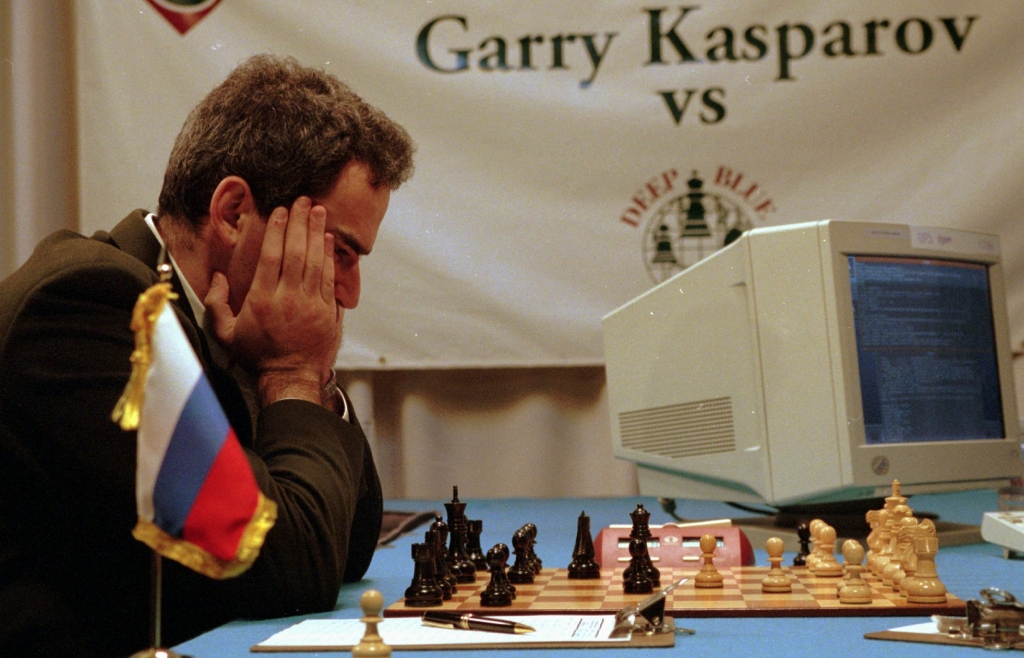
\includegraphics[width=9cm]{img/cap1/chesschallenge}
  \end{center}
  \caption{Gary Kaspárov en uno de sus duelos contra la supercomputadora Deeper Blue.}
  \label{fig:chesschallenge}
\end{figure}

No es el primer deporte que se toma como banco de pruebas. Hace unos años se investigó y se desarrollaron multitud de algoritmos de búsqueda con la excusa del ajedrez. En 1997 la supercomputadora \textit{Deeper Blue} consiguió ganar al campeón del mundo en ese momento, el ruso Gary Kaspárov. En la figura \ref{fig:chesschallenge} se puede ver una instantánea de la partida entre el jugador y la máquina. La forma de interacción con el entorno y las piezas era a través de una persona que introducía en el ordenador los movimientos que realizaba Kaspárov y hacía el movimiento mostrado en la pantalla. \\

El ajedrez y el fútbol son dominios prácticamente opuestos en los que hay que enfrentarse a distintos desafíos para cumplir los objetivos. Las diferencias se pueden ver en la figura \ref{tab:chessvsrobocup}.\\

\begin{figure}[h]
\begin{center}
  \begin{tabular}{| l | l | l |}
    \hline
    & Ajedrez & RoboCup \\ \hline
    Entorno & Estático & Dinámico \\ \hline
    Cambio de estado & Por turnos & Tiempo real \\ \hline
    Visión del problema & Completa & Incompleta \\ \hline
    Percepción/Interacción entorno & A través humano & Sensores y motores \\ \hline
    Control & Centralizado & Distribuido \\ \hline
  \end{tabular}
  \caption{Ajedrez vs Fútbol de robots}
  \label{tab:chessvsrobocup}
\end{center}
\end{figure}

Las diferencias entre los dos deportes saltan a la vista. Un partido de fútbol es un entorno hostil y dinámico donde en unos pocos segundos la situación de juego puede cambiar radicalmente. Las decisiones se tienen que tomar instantáneamente y con los datos disponibles, porque no se tiene una percepción completa del entorno. Toda la información proviene directamente de los sensores. Al ser un juego en equipo también son importantes la información que puedan proporcionar el resto de los robots. En el ajedrez, en cambio, se tiene una visión completa del escenario y el juego es por turnos, por lo que las decisiones no tienen por qué ser instantáneas. Aunque la cantidad de distintos posibles movimientos sea enorme -y de ahí la dificultad del problema-, la interacción y la percepción se hacen a través de una persona y el control es centralizado. \\

Se pueden encontrar infinidad de artículos científicos que utilizan como banco de pruebas la RoboCup. En \cite{MultiObjectsManuela} se desarrolla un algoritmo para hacer el seguimiento de objetos en general en el contexto de la RoboCup. \cite{RobotRecognition} se centra únicamente en el seguimiento de los otros robots que se encuentran en el campo de fútbol. Y por último, en \cite{MultiHypothesis} se presenta un algoritmo para realizar el seguimiento en 2D de objetos en una imagen. Este simplifica la tarea, ya que, al no tener orientación los objetos, no hay rotaciones. Todos estos artículos proponen soluciones al seguimiento de objetos similares a la solución que se ha desarrollado en este proyecto. \\

\section{Estructura del documento}
\label{sec:estructuradeldocumento}

En este documento se describen los aspectos más relevantes del desarrollo del algoritmo. La memoria está dividida en seis capítulos. En este primer capítulo se ha presentado el contexto en el que se va a desarrollar el proyecto. En el segundo capítulo se define el problema concreto, los objetivos y requisitos del proyecto. La infraestructura del software utilizado se expone en el tercer capítulo. El cuarto capítulo describe los detalles técnicos del algoritmo desarrollado. Con el fin de demostrar la validez de la investigación, en el quinto capítulo se adjuntan una serie de experimentos. Por último, el sexto capítulo contiene las conclusiones y se proponen nuevas líneas de investigación.\\
